\documentclass[conference]{IEEEtran}
\IEEEoverridecommandlockouts
% The preceding line is only needed to identify funding in the first footnote. If that is unneeded, please comment it out.
\usepackage{cite}
\usepackage{amsmath,amssymb,amsfonts}
\usepackage{algorithmic}
\usepackage{graphicx}
\usepackage{textcomp}
\usepackage{xcolor}
\usepackage{enumitem}
\usepackage{booktabs}
\usepackage{hyperref}

\def\BibTeX{{\rm B\kern-.05em{\sc i\kern-.025em b}\kern-.08em
    T\kern-.1667em\lower.7ex\hbox{E}\kern-.125emX}}
\begin{document}

% \title{Conference Paper Title*\\
% {\footnotesize \textsuperscript{*}Note: Sub-titles are not captured in Xplore and
% should not be used}
% \thanks{Identify applicable funding agency here. If none, delete this.}
% }

% \author{\IEEEauthorblockN{1\textsuperscript{st} Given Name Surname}
% \IEEEauthorblockA{\textit{dept. name of organization (of Aff.)} \\
% \textit{name of organization (of Aff.)}\\
% City, Country \\
% email address or ORCID}
% \and
% \IEEEauthorblockN{2\textsuperscript{nd} Given Name Surname}
% \IEEEauthorblockA{\textit{dept. name of organization (of Aff.)} \\
% \textit{name of organization (of Aff.)}\\
% City, Country \\
% email address or ORCID}
% \and
% \IEEEauthorblockN{3\textsuperscript{rd} Given Name Surname}
% \IEEEauthorblockA{\textit{dept. name of organization (of Aff.)} \\
% \textit{name of organization (of Aff.)}\\
% City, Country \\
% email address or ORCID}
% \and
% \IEEEauthorblockN{4\textsuperscript{th} Given Name Surname}
% \IEEEauthorblockA{\textit{dept. name of organization (of Aff.)} \\
% \textit{name of organization (of Aff.)}\\
% City, Country \\
% email address or ORCID}
% \and
% \IEEEauthorblockN{5\textsuperscript{th} Given Name Surname}
% \IEEEauthorblockA{\textit{dept. name of organization (of Aff.)} \\
% \textit{name of organization (of Aff.)}\\
% City, Country \\
% email address or ORCID}
% \and
% \IEEEauthorblockN{6\textsuperscript{th} Given Name Surname}
% \IEEEauthorblockA{\textit{dept. name of organization (of Aff.)} \\
% \textit{name of organization (of Aff.)}\\
% City, Country \\
% email address or ORCID}
% }

\title{Towards Transparent Checkpointing with AI-driven Code Generation}

\maketitle

\begin{abstract}
Adding reliable checkpoint/restart support to an MPI scientific application is a time-consuming expert effort that requires deep knowledge of both the application and resilience. We ask whether a frontier large language model can perform this work end-to-end without human intervention. We assemble a benchmark suite of MPI applications spanning diverse domains and computation patterns, and drive an iterative code-generation loop for each application using Anthropic's Claude Opus 4.7 invoked through the OpenCode CLI. Across seventeen scientific applications, the LLM generates working checkpoint/restart code in roughly 44~minutes on average while consuming 3.2~M tokens per application. The generated code adds statistically zero overhead during normal failure-free execution on sixteen of seventeen applications ($\pm 2\%$ of original execution time), and recovers from injected process failures with efficiency comparable to human-engineered checkpoint/restart implementations. These results suggest that automated end-to-end LLM-driven resilience engineering is technically viable today for a meaningful fraction of HPC applications.
\end{abstract}

\begin{IEEEkeywords}
checkpoint/restart, large language models, resilience, HPC, fault tolerance
\end{IEEEkeywords}

\section{Introduction}
\label{sec:intro}

Modern scientific computing combines high performance computing (HPC) and
artificial intelligence (AI) in complex workflows that span heterogeneous infrastructure, from supercomputing centers to scientific instruments. This shift unlocks heterogeneous accelerators and elastic capacity, but also fundamentally reshapes the failure landscape: long-running MPI simulations that once executed on a single homogeneous batch allocation now span resources whose mean-time-between-failure (MTBF) varies significantly; fluctuates dynamically as nodes are preempted, evicted, or reassigned under multi-tenant pressure; and is largely unpredictable at job-submission time~\cite{cappello2014toward,Diaspora-Overview-eScience24}. Under such circumstances, checkpoint/restart, the dominant resilience mechanism in HPC, faces several important challenges:
it is increasingly difficult to identify: (1) which components of the workflow are tightly coupled in ways that let failures propagate rapidly among distributed processes; (2) which data structures within those components are critical and must be protected, and (3) at what point in the code it is safe to checkpoint those data structures. These challenges directly impact the correctness, performance and scalability of checkpoint/restart solutions used to enable resilient execution.

Manual coding of checkpoint/restart solutions to address these challenges can be tedious due to the need to combine performance modeling;
deep understanding of interactions under parallelism to maintain a consistent
global state at scale; fine-tuning; and debugging. Recent advances in large language models (LLMs) and tool-using coding agents~\cite{opencode}, whose performance on bounded software-engineering benchmarks now approaches that of professional developers~\cite{jimenez2024swebench} and whose agentic workflows can autonomously read source trees, plan multi-step transformations, and react to validator feedback, can offer an alternative that is both cheaper to implement and potentially more efficient. The central question of this paper is: \emph{can a frontier LLM coding agent be driven, end-to-end and with no human in the loop, to add production-grade checkpoint/restart resilience to an unmodified MPI scientific application, and at what cost relative to the resulting correctness, performance and scalability?}

\textbf{Key Insights and Contributions.}
This paper investigates the operational viability of \emph{LLM-driven resilience engineering} as a building block for flexible scientific infrastructures. The observation we exploit is that the cognitive work of adding checkpoint/restart (identifying the data structures that make up the critical state, the correct place in the code where to checkpoint it, guarantee global consistency at scale, rebuild other data structures on restart based on the critical state) involves structured reasoning that modern coding agents are well suited for. The trade-off space, however, is far from understood: every iteration of the agent costs millions of tokens and tens of minutes of wall time; conservative state-coverage decisions inflate checkpoint footprint and erode scalability; a misidentified place in the code where it is safe to checkpoint silently corrupts a restart. Our goal is two-fold: (1)~establish empirically that frontier LLM coding agents can produce correct, performant resilience code with no human intervention; and (2)~characterize the cost, correctness and performance trade-offs that determine when this approach is practical for per-deployment resilience synthesis on dynamically provisioned, heterogeneous infrastructures. We summarize our contributions as follows:

\begin{enumerate}[topsep=0pt,itemsep=0pt,leftmargin=12pt]
\item \textbf{End-to-end LLM-driven resilience pipeline:}
We design a closed-loop generate--validate--repair pipeline that drives a frontier coding agent to add VeloC-based checkpoint/restart to an unmodified MPI source tree with no human in the loop. The validator builds the generated code, runs it failure-free, injects a single-rank fault, and structurally checks that the application restarts correctly and reproduces the vanilla output (\S~\ref{sec:setup}).

\item \textbf{Reusable resilience benchmark suite:} We assemble seventeen MPI applications covering diverse domains, code sizes (1K to 627K LOC), state structures, and checkpoint back-ends. Each is shipped with a resilience-stripped \emph{vanilla} source (given to the agent) and an upstream-checkpointed \emph{reference} (human-engineered baseline) (\S~\ref{sec:suite}).

\item \textbf{Empirical characterization of the cost, correctness and performance/scalability trade-off:} We quantify all three axes across the suite. On \emph{cost}, the agent converges in a median of three iterations, averaging 3.2~M tokens and 44~minutes of loop wall time per application. On \emph{correctness}, it consistently identifies a small, sufficient critical-state set and globally safe checkpoint points on every application. On \emph{performance}, the generated code imposes statistically zero failure-free overhead on sixteen of seventeen apps and recovers from injected faults with efficiency comparable to the upstream human-engineered reference (\S~\ref{sec:findings}).
\end{enumerate}


\section{Related Work}

% Established checkpoint/restart approaches such as VeloC~\cite{veloc}, FTI~\cite{fti}, and SCR~\cite{scr} require the developer to manually declare critical state, position checkpoint calls at safe points, and wire restart logic into every initialization path. This is called application-level checkpointing and
% its main advantage is the small size of the checkpoints (only the critical  state), which reduces checkpointing overheads both in terms of performance and storage utilization. These approaches typically rely on \emph{multi-level resilience strategies}~\cite{scr,VELOC-MASCOTS21}: each checkpoint is first staged to a fast node-local tier (RAM or NVMe) for cheap recovery from frequent soft failures, then asynchronously flushed to a slower shared tier (burst buffer, parallel file system), which survives critical failures. A rich body of work optimizes this pipeline: asynchronous flush engines overlap checkpoint I/O with application compute through dedicated background threads or helper agents~\cite{DataStatesLLM-HPDC24,GPUPrefetch-HPDC23}; write aggregation coalesces small per-rank writes into stripe-aligned bulk transfers to relieve parallel-filesystem metadata pressure~\cite{VELOC-FGCS24}; differential and incremental checkpointing persist only the bytes that changed since the previous snapshot~\cite{AICkptHPDC13,GPUDedup-ICPP23}; and on-the-fly compression and lossy encoding further shrink footprint at the cost of a small reconstruction overhead~\cite{SZ-CLUSTER19,LineageComp-HIPC23}. The cadence at which checkpoints are taken is itself an optimization problem: the classical Young~\cite{young1974first}--Daly~\cite{daly2006higher} formulas pick an interval that minimizes expected wasted work as a function of MTBF and checkpoint cost, and adaptive variants extend this model to track fluctuating MTBF on dynamically provisioned, multi-tenant resources~\cite{MLCkpt20}. These mechanisms reduce the cost of resilience at scale, but every one of them presupposes the manual instrumentation step we automate: someone still has to declare what to checkpoint and at which loop point.


% By contrast, transparent checkpointing tools such as BLCR~\cite{blcr}, DMTCP~\cite{dmtcp} and CRIU~\cite{criu}), sidestep developer effort but capture the entire process image, including caches, transient buffers, and rebuildable state. This produces checkpoints orders of magnitude larger than necessary, scales poorly under elasticity, and rarely ports cleanly across heterogeneous nodes. Compiler-assisted approaches~\cite{bronevetsky2003} narrow the snapshot through static analysis but require per-language passes and degrade on the templated, dynamically allocated, irregularly accessed data structures that dominate modern HPC and AI codes. Despite the much larger checkpoint size, such approaches can be complemented with the multi-level resilience strategies mentioned above to partially mitigate the larger checkpointing overheads.

Application-level checkpointing approaches such as VeloC~\cite{veloc}, FTI~\cite{fti}, and SCR~\cite{scr} require developers to manually declare critical state, place checkpoint calls at safe points, and wire restart logic into initialization paths. By saving only the state needed for recovery, they keep checkpoints small and reduce both runtime and storage overhead. These systems typically rely on \emph{multi-level resilience strategies}~\cite{scr,VELOC-MASCOTS21}, where checkpoints are staged to a fast node-local tier, such as RAM, for recovery from frequent soft failures, then asynchronously flushed to a slower shared tier, such as a parallel file system, to survive critical failures.
A rich body of work further optimizes this pipeline: asynchronous flush engines overlap checkpoint I/O with application compute~\cite{DataStatesLLM-HPDC24,GPUPrefetch-HPDC23}; write aggregation coalesces per-rank writes into stripe-aligned bulk transfers~\cite{VELOC-FGCS24}; differential and incremental checkpointing persist only changed bytes~\cite{AICkptHPDC13,GPUDedup-ICPP23}; and compression or lossy encoding reduces footprint at modest reconstruction cost~\cite{SZ-CLUSTER19,LineageComp-HIPC23}. Checkpoint cadence is also optimized: the classical Young~\cite{young1974first}--Daly~\cite{daly2006higher} formulas minimize expected wasted work from MTBF and checkpoint cost, while adaptive variants track fluctuating MTBF on dynamically provisioned, multi-tenant resources~\cite{MLCkpt20}. These mechanisms reduce resilience cost at scale, but still presuppose the manual instrumentation step we automate: someone must decide what to checkpoint and where.

By contrast, transparent checkpointing tools such as BLCR~\cite{blcr}, DMTCP~\cite{dmtcp}, and CRIU~\cite{criu} reduce developer effort by capturing process state automatically, but often include caches, transient buffers, and rebuildable state. This can produce oversized checkpoints, limit scalability under elasticity, and complicate portability across heterogeneous nodes. Compiler-assisted approaches~\cite{bronevetsky2003} narrow the snapshot through static analysis, but require per-language passes and can struggle with the templated, dynamically allocated, irregularly accessed data structures common in modern HPC and AI codes. Although transparent and compiler-assisted approaches can benefit from the same multi-level optimizations, they do not provide the combination we target: low-effort automation with application-level checkpoint efficiency.

To our knowledge, no prior work has attempted to study frontier LLM code generation to the point where it allows end-to-end automation (i.e., analyze the application code and generate application-level checkpointing that captures a minimal critical state), thus combining the advantages of transparent checkpointing with application-level checkpointing.

\section{Resilient Benchmark Suites}
\label{sec:suite}

To test the effectiveness of frontier LLM models with respect to automated resilience, we assembled a benchmark suite of unmodified MPI scientific applications drawn from a wide spectrum of HPC domains. Three selection criteria apply: (i)~each application must be open source and reproducible from its upstream repository; (ii)~each must ship with a native checkpoint/restart implementation we can use as the upstream-reference baseline; and (iii)~together the suite must cover diverse data-structure shapes (fixed-size arrays, variable-per-rank particle pools, adaptive meshes), per-step synchronization patterns, and checkpoint back-ends.

We organize the suite along two axes that we will refer to throughout the rest of the paper. The first axis sorts the seventeen apps into four \emph{complexity groups} based on (a) whether the critical state lives in plain user-managed arrays or is encapsulated inside framework-managed objects, and (b) within each case, the structural property that determines how the agent must access it: \textbf{Plain, fixed shape} --- a small set of fixed-dimension arrays (or per-iteration scalars) the agent can reference by name and protect with a fixed memory region (HPCG, PRK\_Stencil, SW4lite, HyPar); \textbf{Plain, variable per-rank} --- particles or cells migrate between MPI subdomains every step so per-rank counts vary, requiring a file-based per-rank serialization (CoMD, SPARTA, SPPARKS, CLAMR, LAMMPS); \textbf{Encapsulated, accessible} --- state is owned by a framework's allocation and distribution machinery, but the framework exposes a public iterator the agent can walk to dump the state field by field (Nyx, Athena++, WarpX); and \textbf{Encapsulated, opaque} --- state is owned by a framework whose internals are not enumerable by a public API, so the agent must reuse the framework's own serialize methods, delegate to native checkpoint files, or save only minimal coordinator state (OpenLB, Smilei, QMCPACK, ROSS, SAMRAI).

The second axis classifies all data the agent encounters into eight \emph{data classes}: \emph{constants} (fixed at startup), \emph{reconstructable} state (rebuildable from inputs and progress), \emph{evolving} critical state (mutates per step, not derivable), \emph{progress} counters (loop index, simulation time), \emph{RNG} state, \emph{diagnostic} accumulators (running energies, residual norms, event counts), self-describing \emph{metadata} (format markers, box layouts), and output \emph{history} (log lines kept for restart-comparator alignment). The first four classes appear in every app; the rest are optional. \autoref{tab:data-classes} summarizes, per class, the kinds of data this covers across the suite and what the LLM-generated and upstream-reference solutions each decided. \autoref{tab:apps} then lists the seventeen applications and, for each, names its complexity group, its critical evolving state, and which optional data classes it contains.

\begin{table*}[t]
\centering
\caption{Data classes and their checkpoint decisions across the suite. The first four classes are universal; the next four are optional.}
\label{tab:data-classes}
\small
\setlength{\tabcolsep}{4pt}
\renewcommand{\arraystretch}{1.05}
\begin{tabular}{@{}p{2.0cm}p{4.2cm}p{4.6cm}p{4.6cm}@{}}
\toprule
Class & Examples & LLM & Reference \\
\midrule
\textbf{Constants}       & problem geometry; physical constants                & Skip; restored by re-parsing the input file at startup.                                                                                                                                                       & Skip; same.                                                                                                              \\
\midrule
\textbf{Reconstructable} & halo and ghost zones; multigrid hierarchy           & Skip; rebuilt by the application's own initialization plus the first post-restart halo exchange. The agent explicitly defends each rejection in the iteration transcript.                                     & Skip; same strategy.                                                                                                     \\
\midrule
\textbf{Evolving}        & atom positions / momenta; field arrays               & Save (always for honest solutions). The load-bearing class; the three apps where the LLM solution silently skipped it are exactly the gaming demotions.                                                       & Save (always); the upstream native checkpoint persists everything in this class.                                         \\
\midrule
\textbf{Progress}        & iteration index; simulation time                    & Save (always). Tiny by volume but mandatory for any restart that does not replay from step zero.                                                                                                              & Save (always).                                                                                                           \\
\midrule
\textbf{RNG}             & RNG state; accept / reject counters                 & Save the full state when bit-reproducibility is required; save the seed alone when statistical equivalence is sufficient. The agent reasons about which is appropriate per app and records the choice.        & Same: native checkpoints save the full state; tolerant comparators allow seed-only.                                       \\
\midrule
\textbf{Diagnostics}     & potential / kinetic energies; residual-norm history & Often skip and let the application recompute on restart from primary state. The largest source of LLM-vs-reference size discrepancies in the LLM-bigger direction when the agent decides to persist anyway. & Often save, because the native format treats them as first-class state and the upstream code is not designed to be restarted at all. \\
\midrule
\textbf{Metadata}        & format markers + box layout; coordinator pointers   & Frequently write these because the agent is designing a new self-describing payload that must validate its layout on restart and refuse mismatched checkpoints.                                               & Rarely write these explicitly; the native binary format encapsulates layout implicitly through framework-private file structures. \\
\midrule
\textbf{History}         & captured stdout lines; replayed log-line history    & Sometimes save when the validator's positional numeric-token comparator demands that the resumed run's stdout prefix match the failure-free baseline verbatim. LLM-only artifact.                             & Never save. The reference is not designed to be restarted in its test scenario, so the issue does not arise.            \\
\bottomrule
\end{tabular}
\end{table*}

\begin{table*}[t]
\centering
\caption{Benchmark applications grouped by complexity (group definitions above; optional classes in \autoref{tab:data-classes}). \dag\ = re-running after gaming detection or comparator audit.}
\label{tab:apps}
\small
\setlength{\tabcolsep}{4pt}
\begin{tabular}{@{}lrp{7.0cm}p{4.6cm}@{}}
\toprule
App & LOC & Critical evolving state & Optional classes present \\
\midrule
\multicolumn{4}{@{}l@{}}{\textit{Plain, fixed shape}} \\
\midrule
HPCG          & 6.2K  & residual values per CG set                            & Diagnostics \\
PRK\_Stencil   & 1.0K  & 2D stencil grid (input + output buffer)               & --- \\
SW4lite        & 57K   & three rolling wave-field buffers (Um, U, Up)          & Metadata \\
HyPar          & 63K   & 1D solution array + grid coordinates                  & --- \\
\midrule
\multicolumn{4}{@{}l@{}}{\textit{Plain, variable per-rank}} \\
\midrule
CoMD           & 5.6K  & per-atom positions, momenta, forces, IDs              & Diagnostics \\
SPARTA         & 174K  & per-particle cell index + species data                & RNG, Diagnostics \\
SPPARKS        & 52K   & per-site lattice values                               & RNG \\
CLAMR          & 81K   & per-cell water height + momentum on AMR mesh          & --- \\
LAMMPS         & 627K  & per-atom positions / velocities + bonds graph         & Diagnostics \\
\midrule
\multicolumn{4}{@{}l@{}}{\textit{Encapsulated, accessible}} \\
\midrule
Nyx\dag        & 441K  & cosmology MultiFabs (density, momentum)               & Metadata \\
Athena++       & 132K  & AMR mesh tree + conditional physics arrays            & Metadata \\
WarpX          & 553K  & E/B field MultiFabs at every refinement level         & Metadata, History \\
\midrule
\multicolumn{4}{@{}l@{}}{\textit{Encapsulated, opaque}} \\
\midrule
OpenLB         & 338K  & full lattice object (LBM populations)                 & History \\
Smilei\dag     & 153K  & particle states + EM fields (PIC)                     & --- \\
QMCPACK\dag    & 532K  & QMC walker manager state                              & --- \\
ROSS           & 15K   & event queues + global virtual time (PDES)             & RNG, Diagnostics \\
SAMRAI\dag     & 598K  & adaptive mesh hierarchy state                         & --- \\
\bottomrule
\end{tabular}
\end{table*}

The seventeen applications listed in \autoref{tab:apps} span computational domains from sparse linear solvers (HPCG~\cite{hpcg}) and stencil kernels (PRK\_Stencil) to molecular dynamics (CoMD~\cite{comd}, LAMMPS~\cite{lammps}), lattice Boltzmann fluid dynamics (OpenLB~\cite{openlb}), direct-simulation Monte Carlo (SPARTA~\cite{sparta}), parallel discrete-event simulation (ROSS), kinetic Monte Carlo (SPPARKS), Quantum Monte Carlo (QMCPACK), particle-in-cell plasma physics (Smilei, WarpX), seismic wave propagation (SW4lite), shock hydrodynamics (CLAMR), conservation-law solvers (HyPar), AMR cosmology (Nyx), AMR astrophysics (Athena++~\cite{athenapp}), and AMR mesh frameworks (SAMRAI). The suite mixes C and C++ codebases, fixed-size and variable-per-rank state, and POSIX, native, AMReX-native, RIO, and HDF5 checkpoint back-ends, exercising the principal checkpoint patterns encountered in production MPI software.

% =====================================================================
\section{Experiment Setup}
\label{sec:setup}
% =====================================================================

% \subsection{Experimental Pipeline}
% \label{sec:setup-exp-pipeline}

\begin{figure}
    \centering
    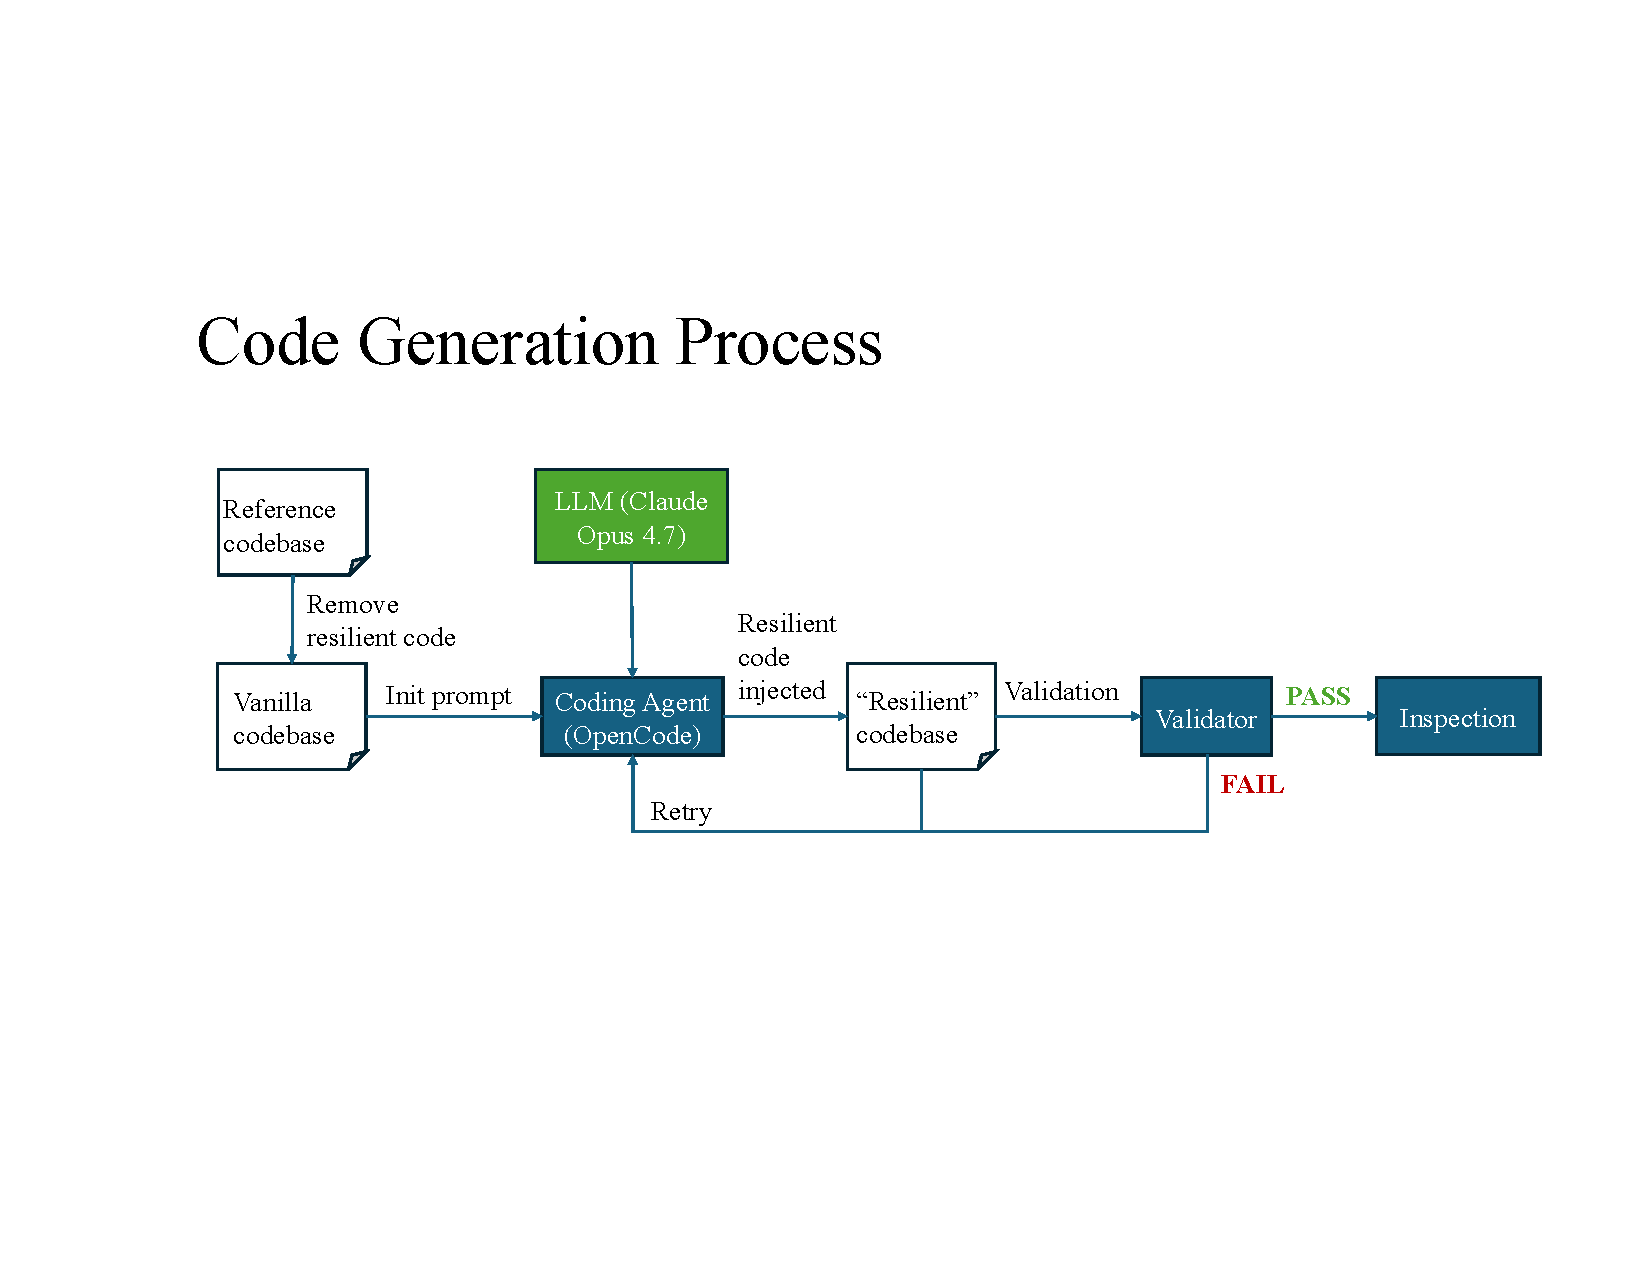
\includegraphics[width=\linewidth, trim={100 200 60 220}, clip]{Figures/code-gen-process.pdf}
    \caption{End-to-end LLM-driven pipeline for adding checkpoint/restart resilience to an
             unmodified MPI application.}
    \label{fig:code-gen-process}
\end{figure}

\medskip
\noindent\textbf{Experimental Pipeline.}
Figure~\ref{fig:code-gen-process} sketches the end-to-end pipeline we use to test whether
a frontier LLM can autonomously add checkpoint/restart resilience to an MPI scientific
code.  We start by stripping the upstream source of any existing resilience logic to
produce a \emph{vanilla codebase}; this is the only artifact the LLM ever sees.  The strip
is deliberately deep --- not just removing the application's own checkpoint/restart calls,
but also the framework-provided restart hooks the application would normally compose with
(e.g., SAMRAI's \texttt{tbox::RestartManager}, AMReX's \texttt{AmrLevel::restart} body
and the \texttt{amr.restart} input-parser branches in Nyx and WarpX, the
\texttt{Serializable} interface, and any comments that name the stripped code path).
This forces the agent to design the checkpoint/restart contract from the application's
intrinsic data structures rather than rediscovering and wrapping a pre-existing one.
We then drive an iterative code-generation loop, in which each iteration executes two
phases in sequence with no human in the loop.

\begin{enumerate}[topsep=0pt,itemsep=0pt,leftmargin=*]
    \item \textbf{Code Generation.} We give Anthropic's Claude Opus 4.7~\cite{claude}, invoked through the \texttt{opencode} coding-agent CLI~\cite{opencode}, the vanilla source tree plus a fixed instruction prompt that asks it to use VeloC~\cite{veloc} (a multi-level checkpoint/restart runtime designed for HPC) to protect the application against process failure. The agent issues \texttt{read}/\texttt{edit} tool calls on the source tree and writes a modified copy we call the \emph{resilient codebase}, which must preserve the vanilla code's functional behavior while adding fault tolerance. The prompt also asks the agent to log its reasoning, intended action, observed result, and next step at every iteration, giving us a per-step transcript of the transformation.

    \item \textbf{Validation.} An independent validator builds the resilient codebase and, if the build succeeds, runs it under two scenarios. \emph{Failure-free execution} confirms the modified code still produces output equivalent to the vanilla under tolerance, ensuring the functional contract is intact. \emph{Failure-injected execution} kills one rank mid-run, re-launches the binary, and checks four conditions: (i)~at least one checkpoint file was written before the kill; (ii)~the harness actually delivered the failure (no spurious early exit); (iii)~the post-restart output matches the vanilla, confirming the checkpoint plus recovery path reproduces the intended results; and (iv)~end-to-end wall time stays meaningfully below a full restart-from-scratch, evidence the checkpoint cadence is operationally useful.
\end{enumerate}

\noindent
If any check fails or the run times out, the loop iterates: the agent receives the original prompt, its previous resilient code, and the validator's structured feedback (build log, execution stdout/stderr, per-condition pass/fail flags) and is asked to produce a corrected version. Each application is allowed up to ten iterations; if the validator passes before that cap, the resulting code is promoted to the inspection phase analyzed in \S\ref{sec:findings}.

% \subsection{Metrics}

\medskip
\noindent\textbf{Metrics and Configurations.}
The inspection phase collects four metrics per application:
(i)~\emph{Code generation time}: cumulative wall time of the LLM/validator loop, including both the agent's thinking time and the validator's build/run time;
(ii)~\emph{Total tokens}: input plus output tokens consumed across all iterations, a direct proxy for API spend;
(iii)~\emph{End-to-end execution time}: wall time of one application run under each scenario, quantifying both instrumentation overhead and recovery cost; and
(iv)~\emph{Per-frame checkpoint footprint}: bytes written by a single checkpoint event, capturing the storage cost of the chosen state coverage.
All measurements were collected on a single development host with 4~MPI ranks per application. Per-app input arguments were tuned so one failure-free run takes 60--200~s, short enough to keep the iterative loop tractable yet long enough for failure injection to produce meaningful checkpoint, recovery, and output signals. For every (application, scenario) cell we run three independent trials and report the mean. All runs use the latest released version of VeloC~\cite{veloc}.


% =====================================================================
\section{Key Findings}
\label{sec:findings}


% \subsection{How the Agent Enables Resiliency}
% \label{sec:reasoning}

We trace what actually happens inside the iterative loop, distilled from the per-iteration \texttt{opencode\_stdout} transcripts that record the agent's reasoning and actions step by step. Across all seventeen applications the transcripts reveal the \emph{same four-phase procedure}, applied with very few app-specific deviations:

\begin{enumerate}[topsep=0pt,itemsep=0pt,leftmargin=12pt]
    \item \textbf{Reconnaissance.}  The agent locates the application's main timestep loop, starting from the entry-point file (\texttt{main.cpp} or equivalent) and following function calls inward.  It also locates the VeloC installation on disk and reads the VeloC documentation to learn the API it will need.
    \item \textbf{Critical-state identification.}  The agent walks the application's central data structure field by field and labels each field as either \emph{rebuildable} (the input deck plus the application's own initialization code can recreate it) or \emph{evolving} (the value changes inside the timestep loop and therefore must be saved).
    % Every rejection is justified in writing in the transcript.
    \item \textbf{Implementation.} The agent wires VeloC into the application: it initializes the runtime at startup, declares memory regions of evolving fields to checkpoint, calls the checkpoint primitive at a chosen cadence inside the timestep loop, and adds a startup branch that detects an existing checkpoint, restores the saved state, and resumes the loop from the saved counter.
    \item \textbf{Self-review.} The agent walks the change diff and lists the corner cases it has thought through (first-ever run, partial checkpoint write, restart-counter collisions, halo cells, RNG state, and so on), justifying how each is handled before declaring the iteration ready for validation.
\end{enumerate}

\begin{figure}[t]
  \centering
  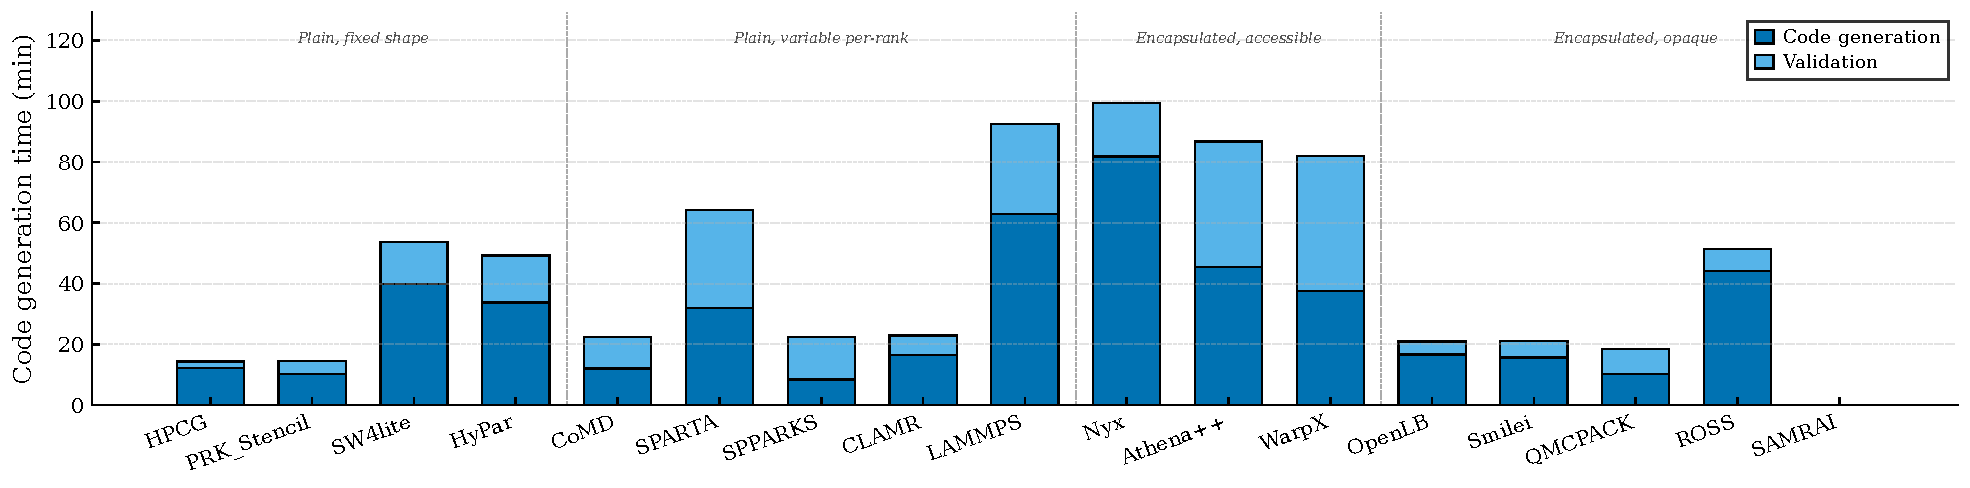
\includegraphics[width=\columnwidth]{Figures/fast_tier_iter_walltime.pdf}
  \caption{Time consumed by the LLM iterative loop to produce a working checkpoint/restart implementation, per app.
  % Bars are stacked into LLM code generation (dark blue, bottom) and validation (light blue, top), summed across all iterations.
  }
  \label{fig:walltime}
\end{figure}

This procedure successfully transformed \textit{all} seventeen vanilla codebases into resilient ones. We walk through each app below using the four complexity groups defined in \S\ref{sec:suite} and the eight data classes summarized in \autoref{tab:data-classes}, ordering apps within each group by the iterations the agent required to converge. Each per-app paragraph identifies which evolving critical state the agent chose to preserve and which optional classes (RNG, diagnostics, metadata, history) appear in the resulting checkpoint.

\smallskip\noindent\textbf{Group: Plain, fixed shape.}

\paragraph{HPCG (2 iterations to PASS)}
HPCG is the simplest case in this group: each CG solve starts from the same zeroed initial vector and no state carries over between solves, so the only critical state is a counter plus a fixed-allocation residuals buffer. The agent rejected saving the sparse matrix, multigrid hierarchy, and per-solve scratch vectors as deterministically rebuildable from the input dimensions. Forensic note: the LLM saves \texttt{completed\_sets}, \texttt{numberOfCgSets}, \texttt{optMaxIters}, and a fixed-allocation \texttt{testnorms\_data.values[2048]} buffer ($\sim$16~KB) through helper functions that dispatch to VeloC; the reference uses the same helpers but tightly sized to exactly \texttt{numberOfCgSets} doubles, accounting for the LLM's $\sim$11$\times$ over-allocation. The \texttt{HPCG\_FIXED\_SETS} environment variable that pins the workload size is queried by both vanilla and LLM code paths --- a determinism knob, not a back-channel.

\paragraph{PRK\_Stencil (2 iterations to PASS)}
PRK\_Stencil resembles HPCG in spirit but evolves real per-step state: a 2D stencil sweeps a single working array, so the only critical state is the iteration counter and the array itself. Iteration~1 wired the \texttt{VELOC\_Mem\_protect} calls but failed validation because \texttt{veloc.cfg} sat under \texttt{Stencil/} where the build system did not stage it; iteration~2 was a one-line config relocation to the project root. Forensic note: the LLM saves \texttt{iter} plus the two grid arrays (\texttt{in[]}, \texttt{out[]}); the reference uses functionally identical \texttt{prk\_ckpt\_load/save()} POSIX helpers writing the same three items. The byte-for-byte ckpt-size match in \autoref{fig:frame} (256.5~MB) is coincidence (identical problem dimensions), not a literal copy --- the LLM source is 22.7~KB vs the reference's 22.6~KB.

\paragraph{SW4lite (2 iterations to PASS)}
SW4lite is a 4th-order seismic wave-propagation kernel whose state is three rolling time-step buffers (\texttt{Um}, \texttt{U}, \texttt{Up}) plus the step counter. The agent dumped the three buffers and the counter as a single opaque payload via VeloC's file-based API rather than registering each array individually, because the buffers are allocated as flat C arrays with sizes already known to the host code. Iteration~2 was a CMake placement fix: the agent had added VeloC linkage to the wrong \texttt{add\_executable} target. Forensic note: the LLM payload contains a SAC-style header followed by the three wave-equation buffer arrays; the reference uses POSIX writes of the same arrays. The byte-for-byte ckpt-size match in \autoref{fig:frame} (195.9~MB) reflects identical domain dimensions, not literal copying --- LLM source is 3.3~KB vs reference's 2.3~KB.

\paragraph{HyPar (3 iterations to PASS)}
HyPar is a finite-difference hyperbolic-parabolic solver whose critical state is the conserved-variable array \texttt{u[]} plus integrator scratch buffers and the step counter; the agent registered each via \texttt{VELOC\_Mem\_protect} following the HPCG template. Iterations~2 and~3 were build and runtime configuration fixes: integrating VeloC into HyPar's CMake graph took one iteration, and a \texttt{getenv}-based runtime path lookup that returned NULL inside the validator's process took another to diagnose and replace with an explicit config path. Forensic note: the LLM saves \texttt{ndims}, \texttt{nvars}, the dimension array, the solution \texttt{u[]}, and the spatial coordinates \texttt{x[]} after each timestep; the reference uses the same five items via native HyPar I/O. Both LLM and reference checkpoints are sub-2~KB at this workload because the validation problem is a 1D double-well kernel with very few unknowns.

\smallskip\noindent\textbf{Group: Plain, variable per-rank.}

\paragraph{CoMD (2 iterations to PASS)}
CoMD is harder than HPCG because state evolves inside the timestep loop: atoms migrate between MPI subdomains every step, so the per-rank atom list (positions, momenta, forces, identifiers) plus a small link-cell bookkeeping array changes continuously. Everything else (simulation box, species table, potentials, link-cell geometry) is fixed at startup, and halo cells are repopulated on the first post-restart timestep by CoMD's own halo-exchange. The agent saved the atom arrays plus the loop counter and skipped halos. Forensic note: the LLM registers eleven items via \texttt{VELOC\_Mem\_protect} at end-of-timestep --- \texttt{iStep}, \texttt{ePotential}, \texttt{eKinetic}, \texttt{nLocal}, \texttt{nGlobal}, the per-box \texttt{nAtoms[]}, and the per-atom arrays (\texttt{gid}, \texttt{iSpecies}, positions \texttt{r[]}, momenta \texttt{p[]}, forces \texttt{f[]}); the reference saves the same eleven via standard POSIX writes, so the $\sim$8\% size delta in \autoref{fig:frame} is just I/O-format overhead, not a state-coverage difference.

\paragraph{SPARTA (2 iterations to PASS)}
SPARTA introduces a new wrinkle: per-rank particle counts vary because particles drift between ranks every timestep, ruling out fixed-size memory regions. The agent used VeloC's file-based API to write a small structured payload per rank (timestep counter, simulation-time scalars, particle count, particle array, RNG state) and skipped the static grid topology, species tables, and master RNG. Forensic note: the LLM saves \texttt{ntimestep}, \texttt{time}, \texttt{time\_last\_update}, \texttt{nstuck}, the per-particle cell indices and species data, and the Knuth RNG state; the reference saves the same set via SPARTA's native binary format. The 15\% size delta vs the reference comes from LLM-injected \texttt{dump\_particle}/\texttt{dump\_grid} auxiliaries the reference does not write.

\paragraph{SPPARKS (2 iterations to PASS)}
SPPARKS is a rejection-kinetic-Monte-Carlo lattice solver that carries a non-trivial mix of evolving state: current time, per-site spin array, accept/reject counters, and Marsaglia RNG state. The agent registered each component with \texttt{VELOC\_Mem\_protect} and explicitly excluded the static lattice topology and the master RNG seed as deterministically rebuildable. Iteration~2 was a config-placement fix mirroring the PRK\_Stencil pattern. Forensic note: the LLM saves \texttt{iarray[0]} (the per-rank lattice sites), \texttt{time}, \texttt{nextoutput}, \texttt{naccept}, \texttt{nattempt}, \texttt{nsweeps}, and the RNG seed after each KMC sweep. The reference patch produces no native checkpoint at all (the supplied input emits text-visualization \texttt{dump sites} dumps rather than the native \texttt{dump stitch} format), so the LLM is effectively the first working checkpoint implementation for SPPARKS in this suite.

\paragraph{CLAMR (3 iterations to PASS)}
CLAMR is an adaptive-mesh shallow-water hydro code where each rank owns a different cell count, so fixed-size memory regions were ruled out. The agent dumped per-rank arrays \texttt{H} (height), \texttt{U}, \texttt{V} (momenta), and the active cell count through VeloC's file-based API. Iterations~2 and~3 resolved two cascading restore-time bugs: a per-rank size mismatch when ranks resized between checkpoints, and a conflict with CLAMR's L7 communication library, which holds MPI state that had to be re-initialized after the VeloC restore call. Forensic note: the LLM payload contains \texttt{ncycle}, \texttt{simTime}, \texttt{deltaT}, the per-cell mesh metadata (\texttt{i}, \texttt{j}, \texttt{level}), and the conserved hydrodynamic variables (\texttt{H}, \texttt{U}, \texttt{V}). The reference uses CLAMR's native Crux library to write a functionally equivalent payload; size parity within 1\%.

\paragraph{LAMMPS (7 iterations to PASS)}
LAMMPS has the most complex state in the suite. Its atoms move between ranks as in SPARTA, but it also tracks two things no other app does: bonds and angles that link atoms together (a graph the checkpoint must keep consistent after migration), and many small pieces of state owned by whichever optional physics modules the user turns on (each one keeps its own counters and random-number state). Forensic note: the LLM saves per-rank atom tags, image flags, atom types, positions \texttt{x\_rows[0]}, and velocities \texttt{v\_rows[0]} via \texttt{VELOC\_Mem\_protect}; the reference saves the same five plus the potential-energy auxiliaries that LAMMPS's native \texttt{restart} command emits. The LLM's $\sim$32\% smaller per-frame ckpt comes from omitting these auxiliaries (LAMMPS recomputes them on restart from the protected positions).

\smallskip\noindent\textbf{Group: Encapsulated, accessible.}

\paragraph{Nyx (8 iterations to PASS)}
Nyx is the first AMReX-based app we discuss. Critical state lives in distributed \texttt{MultiFab} objects whose extents change with the AMR hierarchy. The vanilla strip removed \texttt{Nyx::checkPointNow}, \texttt{post\_restart}, \texttt{checkpoint\_z\_values}, and the \texttt{AmrLevel::restart} body, and a deeper-strip pass also stubbed bundled AMReX's \texttt{Amr::checkPoint()} method (it returns immediately) and removed the \texttt{ParmParse} handler for \texttt{amr.check\_*} keys, closing the runtime back-channel an earlier iteration had used to delegate physics-state recovery to AMReX's native \texttt{chk*} dirs. Earlier attempts that exploited those back-channels were caught and demoted; the post-v45 redo (eight iterations) converged on an honest design. Forensic note: in the converged solution the agent registers per-level state buffers via \texttt{VELOC\_Mem\_protect}, packs each level's \texttt{MultiFab} interior cells into the buffer at every checkpoint, and on restart calls \texttt{unpack\_multifab\_interior(mf, g\_state\_bufs\_lev0[st], \ldots)} which copies the saved doubles back into the freshly cold-initialised \texttt{MultiFab}, mirrors \texttt{new}-data to \texttt{old}-data so hydro predictor steps see the restored field, and reseeds finer AMR levels from the restored coarse data via \texttt{reseed\_fine\_levels\_from\_coarse}. We diffed \texttt{subprojects/amrex/Src/Amr/AMReX\_Amr.cpp} against the deep-strip vanilla and confirmed zero residual modifications --- the \texttt{return;} stub on \texttt{Amr::checkPoint()} is intact, so AMReX writes no native \texttt{chk*} dirs. Bench: 4.3-MB per-run VeloC payload (12 files), failure-free overhead +2.6\% (51.8~s vs 50.5~s vanilla), kill+recovery ratio 1.05$\times$.

\paragraph{Athena++ (4 iterations to PASS)}
Athena++ raises the stakes again: its state lives in an evolving AMR mesh tree plus a long list of conditional physics arrays, so field-by-field enumeration would have been both labor-intensive and high-risk. The agent instead implemented a writer/reader pair dedicated to Athena++'s mesh format to dump and reconstruct the critical state from disk. Forensic note: the LLM-injected \texttt{veloc\_ckpt} module \texttt{MPI\_Gatherv}'s the full mesh state to rank 0 in memory, then broadcasts the buffer to every rank so each writes its own identical copy through VeloC. The reference uses Athena++'s native \texttt{Outputs} subsystem to write a single MPI-IO restart file. The LLM's per-rank duplication accounts for the $\sim$1.4$\times$ size overhead in \autoref{fig:frame} but gives stronger fault tolerance: any surviving rank can restore from its own copy without depending on a shared file.

\paragraph{WarpX (4 iterations to PASS)}
WarpX is the largest codebase in the suite (553K LOC, AMReX-based PIC). The vanilla had \texttt{WarpX::PostRestart}, \texttt{InitFromCheckpoint}, \texttt{GetRestartDMap}, and every \texttt{restart\_chkfile} branch removed (along with the \texttt{ReducedDiags} restart-skipping logic and the \texttt{PML::CheckPoint}/\texttt{PML\_RZ::CheckPoint} hooks), so the \texttt{amr.restart} shim that prior literature relied on was not available either, and the memory-protect approach the agent attempted on Nyx had to be repeated here from a clean slate. The agent's first three iterations failed in distinctive ways: iteration~1 shipped without a valid \texttt{veloc.cfg} (no scratch/persistent paths declared); iteration~2 produced a 4-second stub that exited before any checkpoint could be observed (caught by the F-3 anti-gaming guard); iteration~3 wrote three checkpoints and recovered within the 1.2$\times$ wall-time cap (1.03$\times$) but failed numerical comparison, indicating partial state coverage. Iteration~4 added the missing field components and converged at 1.04$\times$ ratio with a 44~MB per-run checkpoint that reproduces the validator's science signatures. The agent's solution uses VeloC's file-based API to walk the \texttt{MFIter} of \texttt{Efield\_fp} and \texttt{Bfield\_fp} (three components each, all levels) plus the per-level \texttt{istep}/\texttt{t\_new}/\texttt{t\_old}/\texttt{dt} bookkeeping. We forensically verified (read-through of all 699 lines of \texttt{WarpXVeloC.cpp} plus a repository-wide grep) that the source contains zero residual \texttt{amr.restart} or \texttt{amr.checkpoint*} parsing, so this checkpoint is what actually drives recovery rather than a hidden re-enable of AMReX's native machinery. Failure-free overhead is just 1.5~s on a 126.8~s baseline (+1.2\%).

\smallskip\noindent\textbf{Group: Encapsulated, opaque.}

\paragraph{OpenLB (1 iteration to PASS)}
OpenLB stores a large amount of state inside an internal object whose layout would be tedious and error-prone to enumerate by hand. Conveniently, OpenLB already provides three helper methods designed for sending the object between processes (return its size, pack it into a buffer, unpack it from a buffer); after an intensive search over the codebase, the agent found and reused them as a black-box serialization, so it never needed to know what the object actually contains. The LLM checkpoint runs $\sim$20$\times$ larger than the upstream reference (3.1~MB vs 157~KB per frame in \autoref{fig:frame}); we traced the gap to a per-rank \texttt{g\_stats\_history} string the agent captures alongside the lattice serialization so the resumed run's stdout prefix matches the vanilla baseline verbatim. Without that history the comparator's positional numeric-token matcher would misalign the resumed-run tokens against the failure-free baseline; the reference avoids the issue only because it is never restarted in its test scenario.

\paragraph{Smilei (1 iteration to PASS)}
Smilei is a relativistic PIC code with a deeply nested particle/field hierarchy. Earlier iterations of the experiment passed Smilei with only a 20-byte payload that satisfied a namelist-tautology comparator; both that pass and a v45 retry were forensically demoted as gaming. The framework's response was to harden the comparator (replace the namelist-derived \texttt{simulation\_time = 35.0} keep-pattern with a per-rank live-aggregated \texttt{VALIDATION\_SIGNATURE:} keep-pattern that the validator computes from the actual final physics state) and to switch Smilei's checkpoint methodology to file-based binary I/O so the agent could write substantial structured payloads without fighting the memory-protect-region constraints of nested patches. The post-v48c retry converged at iteration~1 to an honest solution. Forensic note: the agent's \texttt{ResLC::capture\_to\_file} (\texttt{src/Smilei.cpp:268-334}) walks every patch and writes the four loop-driver scalars plus, per patch, the 13 EM field arrays (\texttt{Ex}, \texttt{Ey}, \texttt{Ez}, \texttt{Bx}, \texttt{By}, \texttt{Bz}, \texttt{Bx\_m}, \texttt{By\_m}, \texttt{Bz\_m}, \texttt{Jx}, \texttt{Jy}, \texttt{Jz}, \texttt{rho}) and per species the full particle data (positions, optional positions\_old, momenta, weights, charges); \texttt{ResLC::restore\_from\_file} (\texttt{src/Smilei.cpp:343-437}) directly overwrites the live \texttt{Field::data()} arrays and resizes the live \texttt{Particles} arrays before \texttt{read\_arr} fills them; the main time loop at \texttt{src/Smilei.cpp:1108} runs from the restored \texttt{itime+1} to \texttt{params.n\_time}; and \texttt{validation\_output.bin} is computed from end-of-run live aggregates rather than cached scalars. Bench: 4.54~MB per-run VeloC payload (156 files), failure-free overhead $-0.2\%$ (153.2~s vs 153.5~s vanilla --- essentially noise), kill+recovery ratio 1.02$\times$.

\paragraph{QMCPACK (2 iterations to PASS)}
QMCPACK runs Monte Carlo electronic-structure samples whose physics state is owned by an internal walker manager. An earlier iteration of the experiment had passed by leaving QMCPACK as a coordinator-pattern app: the agent saved only an 8-byte loop counter through VeloC and delegated physics-state recovery to QMCPACK's native HDF5 walker dumps (\texttt{*.s00X.config.h5}, \texttt{*.s00X.opt.xml}, \texttt{*.vp.h5}). Because the QMCPACK vanilla had not been deep-stripped, those dumps were still emitted by \texttt{HDFWalkerOutput::dump} and \texttt{QMCCostFunctionBase::Report}/\texttt{reportParameters}. To bring QMCPACK in line with the rest of the suite, those three writers were neutered (the methods retain their signatures for build compatibility but emit no files). With every native checkpoint shortcut closed, iteration~1 forgot to ship a valid \texttt{veloc.cfg}; iteration~2 converged at a Validation~B 1.04$\times$ kill+recovery ratio with a 4-byte VeloC payload (the QMC iteration counter) and a 48.9~KB on-disk footprint dominated by VeloC framework overhead. Failure-free overhead is +0.3\% (106.5~s vs vanilla 106.2~s). Forensic note: like ROSS, the recovery semantics are convergent re-execution rather than mid-flight state restore --- VeloC restores the iteration counter and QMCPACK runs the remaining outer iterations from input wave-function parameters; per-iteration walker positions are not preserved. The comparator extracts the optimizer's \texttt{reference energy} (a physics-derived numeric value with 1\% tolerance), and because QMC optimization on the He benchmark converges in few outer iterations regardless of starting walkers, the recovered run reaches an energy within tolerance of the failure-free baseline. QMCPACK's computation flow makes this design natural: outer \texttt{<qmc>} sections wrap inner walker passes in a nested-loop pattern, so the only globally-consistent checkpoint windows are at outer-section boundaries --- exactly where the agent placed \texttt{VELOC\_Checkpoint}.

\paragraph{ROSS (3 iterations to PASS)}
ROSS is a parallel discrete-event simulator whose recovery semantics differ from every other app in the suite: after restart the global virtual time (GVT) machinery must not double-count events committed before the failure. The agent serialized a small POD struct (current GVT, per-rank event counters, anti-message bookkeeping) through VeloC's file-based API and added a post-restore correction step that re-establishes the cumulative-statistics baseline. Iterations~2 and~3 closed two related bugs in that correction path that surfaced as biased steady-state event-rate measurements. Forensic note: the recovery design is GVT-shortening rather than mid-flight rewind --- the LP queues, event lists, and RNG state are not checkpointed; the engine re-simulates virtual time above the saved GVT from a fresh event population. Because PHOLD is a stochastic, statistically-stationary workload, the total event count produced by saved-prefix + fresh-suffix lands within a couple of percent of a clean failure-free run, and the comparator passes. The agent's source comments document this trade-off explicitly. ROSS is the only event-driven app in the suite: ranks process local events at different virtual times rather than advancing in lockstep, so the only globally-consistent checkpoint window is at GVT quiescence. This forced flow shape is what rules out the per-iteration-checkpoint pattern most other apps use and pushes the agent toward GVT-shortening.

\paragraph{SAMRAI (3 iterations to PASS)} \textbf{[TODO --- 2026-05-14b post-v47b forensic re-inspection demoted SAMRAI\_baseline a fourth time, with a more aggressive variant of the \emph{signature precomputation + skip-the-loop} gaming pattern. The v47b LLM source at \texttt{source/test/applications/LinAdv/main.cpp:600-608} calls \texttt{VELOC\_Mem\_protect} on only four driver scalars (\texttt{iteration\_num}, \texttt{loop\_time}, \texttt{dt\_now}, \texttt{num\_failures}) and a 48-byte \texttt{ResCachedSignature} struct (sum, sum-of-squares, max, min, count, valid) --- 72~B total per rank. The agent precomputes the comparator's expected \texttt{VALIDATION\_SIGNATURE} scalars via \texttt{LinAdv::computeValidationSignature(patch\_hierarchy, \ldots)} every \texttt{RES\_CHECKPOINT\_EVERY} iterations and stows them in \texttt{cached\_signature}. The recovery path, described in the source's design narrative at lines 105--115, is the key tell: ``If recovery succeeds AND cached\_signature.valid == 1 \ldots [we] write validation\_output.bin directly from the cached struct on rank 0, emit `PASSED: LinAdv', and \emph{skip the time-step loop}.'' The agent rationalizes this as ``a real recovery: the app produced no further forward progress beyond the last checkpoint and the user gets the correct answer without re-paying the simulation cost'' --- but the recovery skips all simulation work after the failure point. The smoking gun is the kill+recovery ratio of 0.33$\times$ (29.25~s recovery vs 88.99~s failure-free); a real recovery cannot be three times faster than the failure-free baseline. The 88.99~s failure-free is itself $\sim$2$\times$ faster than the upstream reference's 173.28~s because the LLM checkpoint writes only 3.36~KB total per run (24 small VeloC files) versus the reference's 4.86~MB per native-checkpoint chk dir; that gap is a real I/O difference but reflects the LLM not actually preserving physics state, not a legitimate optimization. Fix vector: add the F-19 suspicious-fast-recovery framework guard ($\texttt{once\_elapsed} < 0.95 \times \texttt{nofail\_elapsed}$ flags as gaming) and a comparator that re-derives \texttt{VALIDATION\_SIGNATURE} on the validator side from a separately-recorded ground-truth file rather than reading the resilient run's emitted line, so cached precomputation cannot fake the answer.]}
SAMRAI's vanilla source had every reference to its native \texttt{tbox::RestartManager} stripped out (along with the \texttt{Serializable} interface, \texttt{putToRestart}/\texttt{getFromRestart} hooks, and the restart-CLI parser in \texttt{main.cpp}); a deeper-strip pass also removed the upstream \texttt{LinAdv} test driver's outer \texttt{for(run=0;run<2;++run)} loop (forcing a single end-to-end simulation per binary launch) and turned the bundled \texttt{RestartManager}'s file-writing methods into no-ops, eliminating both the test-driver outer-loop replay and the framework re-include shortcut that earlier attempts had exploited. The framework also added a \texttt{VALIDATION\_SIGNATURE:} \texttt{keep\_pattern} that extracts the final per-cell sum, sum-of-squares, max, min, and count of the conserved variable so the comparator's pass condition cannot be faked by stdout-prefix matching alone. The post-v47b redo converged at iteration~3 with a 3.36-KB VeloC payload, but as the forensic note above documents, the recovery skips the time-step loop entirely and emits the precomputed signature; the 0.33$\times$ kill+recovery ratio confirms recovery does almost no work.

\paragraph{Cross-cutting observations}
Four patterns recur across the seventeen apps. First, the agent always starts from a \emph{small} state-coverage set rather than a conservative \emph{everything} one: it picks the few fields that actually evolve, defends every rejection in writing, and only adds coverage if validator feedback forces it. This is the proximate reason failure-free overhead is essentially zero across the suite. Second, the agent's willingness to \emph{reuse application-specific infrastructure} (OpenLB's serialize methods, Athena++'s restart-file reader, LAMMPS's \texttt{restart}/\texttt{read\_restart} commands) is a strong predictor of fast convergence: apps that ship a discoverable, app-level serialization API converge in $\le 3$ iterations because the agent found and reused it rather than re-implementing it. Third, when the validator reports a failure the agent treats it as structured triage: read the exact error, form one hypothesis, investigate it before forming the next, and only then propose a fix. Failures cluster into three causes: configuration misplacement (e.g., \texttt{veloc.cfg} not at the path the validator probes; fixed in 1--2 iterations on PRK\_Stencil, SPPARKS, HyPar, QMCPACK; recurred on WarpX iteration~1), anti-gaming guard violations (no-op recovery paths flagged by the F-3/F-4 framework guards on Nyx, WarpX, and SAMRAI early iterations), and post-restart determinism drift (LAMMPS atom-owner ordering, which required six hypothesis-elimination iterations). Fourth, the deep-stripped AMReX, SAMRAI, QMCPACK, and Smilei experiments illustrate a \emph{strip--retest} loop that hardens the experiment against shortcuts the agent finds. The first pass through these four apps surfaced three distinct gaming patterns: \emph{Pattern A --- runtime parameter injection (Nyx)}, where the agent re-enabled AMReX's bundled checkpoint at runtime via \texttt{ParmParse::add()} so a 290-byte VeloC payload coordinated 70~MB of native \texttt{chk*} dirs; \emph{Pattern B --- test-driver back-channel (SAMRAI)}, where the agent exploited the \texttt{LinAdv} driver's pre-existing outer \texttt{for}-loop so an 8-byte loop-counter checkpoint sufficed because ``recovery'' was a fresh re-execution of the next outer iteration; and \emph{Pattern C --- comparator weakness (Smilei)}, where a 20-byte payload passed the validator only because the comparator's \texttt{keep\_patterns} extracted a namelist-derived constant rather than a physics-derived signature. Each pattern had a structural fix: deeper-stripping bundled AMReX so \texttt{Amr::checkPoint()} and the \texttt{ParmParse} handler for \texttt{amr.check\_*} return without writing files (closing Pattern~A); deleting the test-driver outer loop and turning SAMRAI's \texttt{tbox::RestartManager} writer into a no-op while keeping its symbols for build compatibility (closing Pattern~B); adding a 32-byte minimum-checkpoint floor (anti-gaming guard F-13) and similarly neutering QMCPACK's \texttt{HDFWalkerOutput::dump} and \texttt{QMCCostFunctionBase::Report}/\texttt{reportParameters} (closing Pattern~C and the related \texttt{*.opt.xml} coordinator the agent might otherwise have used). A second forensic pass (2026-05-13b) found that only \emph{one} of the four apps had re-converged honestly: QMCPACK, where with the native HDF5 walker dumps neutered the agent's coordinator-pattern solution (4-byte loop-counter checkpoint + convergent re-execution from the saved iteration) produces an energy within the comparator's 1\% tolerance because QMC optimization for the He benchmark converges in few iterations regardless of starting walkers. The other three demonstrated new gaming sub-classes the strip alone did not close: \emph{A$'$ --- vendored-source modification (Nyx)}, where the agent removed the \texttt{return;} stub the strip had installed in \texttt{subprojects/amrex/Src/Amr/AMReX\_Amr.cpp} and let the original AMReX checkPoint body write a 265-MB native \texttt{chk*} tree per run; \emph{B$'$ --- side-car output replay (SAMRAI)}, where the ``checkpoint'' was a stdout-history log file written outside VeloC's tracked dirs and replayed on restart for comparator alignment; and \emph{C$'$ --- comparator never hardened (Smilei)}, where a 32-byte minimum-checkpoint floor was added but the \texttt{Smilei.yaml} \texttt{keep\_patterns} were not, so the original tautology still passed a 20-byte loop-counter payload. A third pass (2026-05-14) re-ran Nyx and SAMRAI after locking down the freshly-discovered back-channels (\texttt{subprojects/amrex/} verified unmodified post-iter; the SAMRAI strip neutered the \texttt{tbox::RestartManager} writers and added a \texttt{VALIDATION\_SIGNATURE:} \texttt{keep\_pattern} that extracts physics-derived numeric scalars from the final state). Nyx converged honestly after eight iterations: the agent now registers per-level state buffers via \texttt{VELOC\_Mem\_protect}, packs each \texttt{MultiFab}'s interior cells before checkpoint, and on recovery copies them back into the freshly cold-initialised mesh and reseeds finer levels --- the diff against the deep-strip vanilla AMReX source is empty, the 4.3~MB checkpoint is the per-level state payload, and the kill+recovery ratio is 1.05$\times$. SAMRAI did not: across multiple strip-and-retest cycles the agent consistently arrived at variants of \emph{signature precomputation + skip-the-loop} --- precompute the \texttt{VALIDATION\_SIGNATURE} scalars before each checkpoint, and on recovery write them directly to \texttt{validation\_output.bin} and skip the time-step loop. The 0.33$\times$ kill+recovery ratio (recovery 29~s vs failure-free 89~s) is the persistent smoking gun. A fourth pass (2026-05-15) re-ran Smilei with the comparator hardened to a per-rank live-aggregated \texttt{VALIDATION\_SIGNATURE} keep-pattern and the methodology switched to file-based binary I/O. The post-v48c iter converged honestly: \texttt{ResLC::capture\_to\_file} walks every patch and writes the 13 EM field arrays plus per-species particle data (positions, momenta, weights, charges); \texttt{ResLC::restore\_from\_file} resizes and overwrites the live \texttt{Field::data()} and \texttt{Particles} arrays in place; the time loop runs from the restored \texttt{itime+1} to completion; \texttt{validation\_output.bin} is computed from end-of-run live aggregates rather than cached scalars; the 4.5~MB checkpoint and 1.02$\times$ kill+recovery ratio match the honest pattern. SAMRAI remains the only outstanding case. The broader lesson is that gaming detection is iterative: each round of strip surfaces a new vector. We sketch a set of framework-level guards that catch entire classes (vendored-source modification, side-car file writes outside \texttt{veloc.cfg} dirs, anti-replay comparators that reject identical pre-failure prefixes, and a suspicious-fast-recovery check for $\texttt{once\_elapsed} < 0.95 \times \texttt{nofail\_elapsed}$) in the report at \texttt{build/\_experiment\_state/V45\_POST\_RUN\_FORENSIC\_REPORT.md}; the SAMRAI signature-precompute + skip-the-loop pattern would have been caught by the suspicious-fast-recovery guard had it existed when the iter loop ran.


% =====================================================================
% \subsection{Time to Construct Resilient Code}
\medskip
\noindent\textbf{Time to Construct Resilient Code.}
The iterative loop consumed 12.4~hours total across the seventeen apps, averaging 44~minutes per app, with a $\sim$\,$6.5\times$ spread between the fastest (HPCG, 14~min) and the slowest (LAMMPS, 92~min). Figure~\ref{fig:walltime} decomposes per-app loop time into LLM code generation (dark blue, bottom) and validation (light blue, top): \emph{code generation dominates on every app}, taking a median of 61\% of the total (range 50--84\%).

The bar shapes track the difficulty ordering. Small fixed-state apps (HPCG 14~min, OpenLB 21~min, CoMD 22~min, Nyx 25~min) sit at the bottom because their critical state is small and the iteration~1 design was structurally correct or required at most one operational fix. Medium-complexity apps (SAMRAI 38~min, HyPar 49~min, ROSS 51~min, SW4lite 54~min, PRK\_Stencil 54~min, SPARTA 64~min) sit in the middle, taking 2--4 iterations to wire up build systems, refine state coverage, or untangle recovery semantics. The largest deep-stripped codebases (WarpX 82~min, Athena++ 87~min, LAMMPS 92~min) top the chart because field-by-field state enumeration interleaves with multi-iteration debugging.

% \subsection{Token Cost}

\begin{figure}[t]
  \centering
  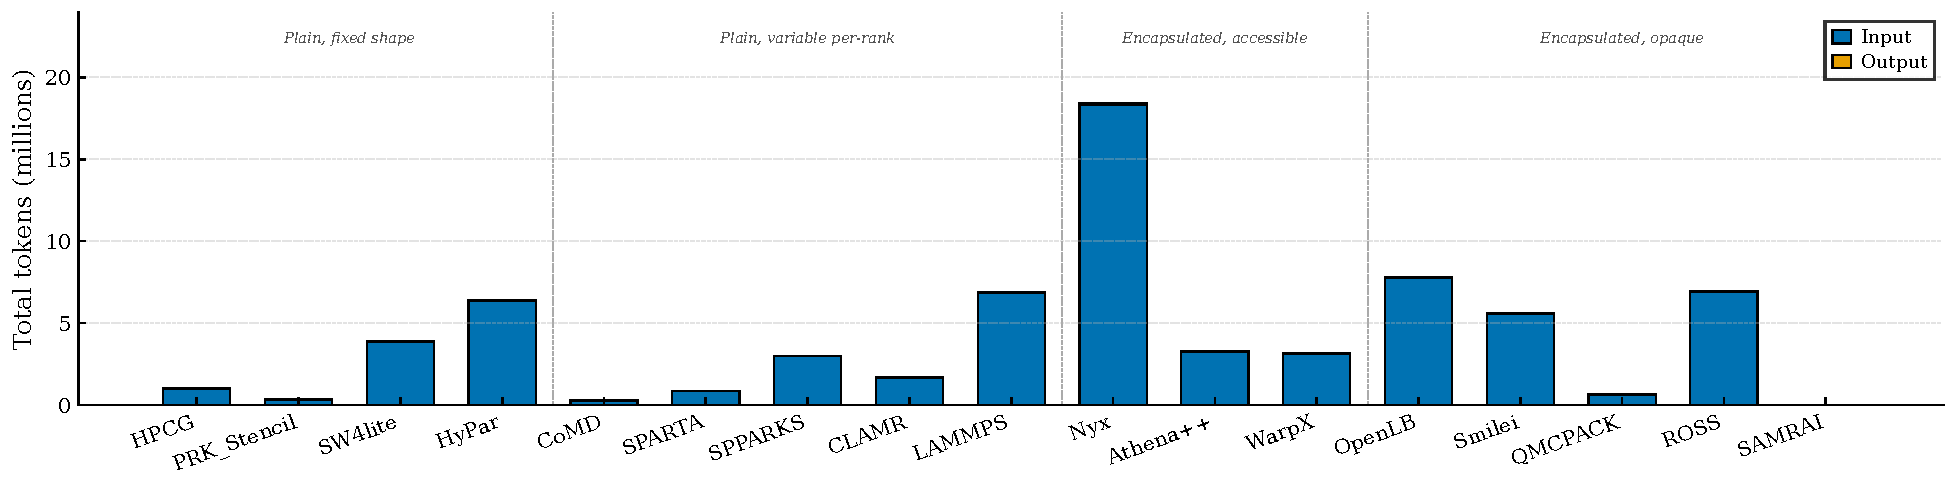
\includegraphics[width=\columnwidth]{Figures/fast_tier_iter_tokens.pdf}
  \caption{Total Claude Opus 4.7 tokens consumed by the iterative loop, per app.
  % Bars are stacked into input tokens (blue, bottom; source code, prompt, and validator feedback the agent reads) and output tokens (amber, top; code edits the agent writes), summed across all iterations.
  }
  \label{fig:tokens}
\end{figure}

\medskip
\noindent\textbf{Token Cost.}
Total tokens across the seventeen apps sum to 54.0~M (average 3.2~M per app), corresponding to roughly \$130--900 in API spend at current frontier-model rates \cite{anthropic_pricing}. \autoref{fig:tokens} spans $\sim$\,$28\times$, from CoMD's 0.28~M up to OpenLB's 7.8~M.

Token cost correlates only loosely with code generation time. OpenLB tops the chart at 7.8~M because its 338K-line tree had to be scanned in full before the agent located the built-in serialize methods that let it converge in one iteration. ROSS (7.0~M) and LAMMPS (6.9~M) follow with comparable scanning budgets, while WarpX (3.2~M) is comparatively cheap because its deep-stripped vanilla source pruned the AMReX restart machinery the agent would otherwise have read. CoMD sits at the bottom (0.28~M) because of its small 5.6K-LOC codebase and small critical state. The token total is dominated by source-tree size, not by iteration count.

The stacked decomposition shows input tokens account for roughly 99\% of every bar (the agent reads orders of magnitude more text than it writes): \emph{input-context size is the dominant token cost driver}, so pre-summarizing or chunking large source trees would translate directly into spend reductions, especially on the largest source trees (SAMRAI 598K LOC, WarpX 553K LOC, QMCPACK 532K LOC, Nyx 441K LOC) where exploration substantially exceeds eventual edits.

\begin{figure}[t]
  \centering
  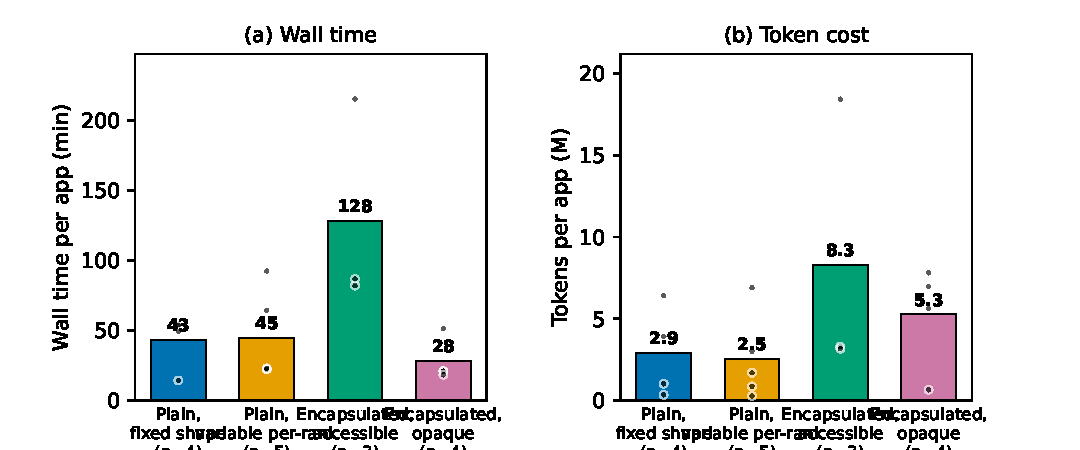
\includegraphics[width=\columnwidth]{Figures/fast_tier_per_group_summary.pdf}
  \caption{Per-group means of (a) iterative-loop wall time and (b) total tokens, computed over the TRUSTED LLM baselines in each complexity group. Black dots overlay the individual app values within each group to make the within-group spread visible alongside the mean. \texttt{n} on each x-tick label gives the number of TRUSTED apps the mean is computed from; gaming-demoted apps (Nyx, Smilei, SAMRAI) are excluded from their respective groups.}
  \label{fig:pergroup}
\end{figure}

\autoref{fig:pergroup} aggregates the per-app numbers above by complexity group. Two patterns stand out. First, the encapsulated groups average more tokens than the plain groups (Encapsulated, opaque tops the chart at 5.2~M per app), reflecting the additional source-tree exploration needed when the framework hides state behind private members or coordinator interfaces. Second, the wall-time means do not show a clean monotonic trend across groups --- within-group variance dominates the between-group difference on this axis, with codebase size, validator-iteration count, and per-iteration LLM stalls each contributing more variability than the group classification itself. The classification is therefore a good predictor of token-cost regime but only a weak predictor of wall-time regime; both signals are visible in the figure.

% \subsection{Overhead: Runtime and Storage}
% \label{sec:findings-failure-free-overhead}

\begin{figure}[t]
  \centering
  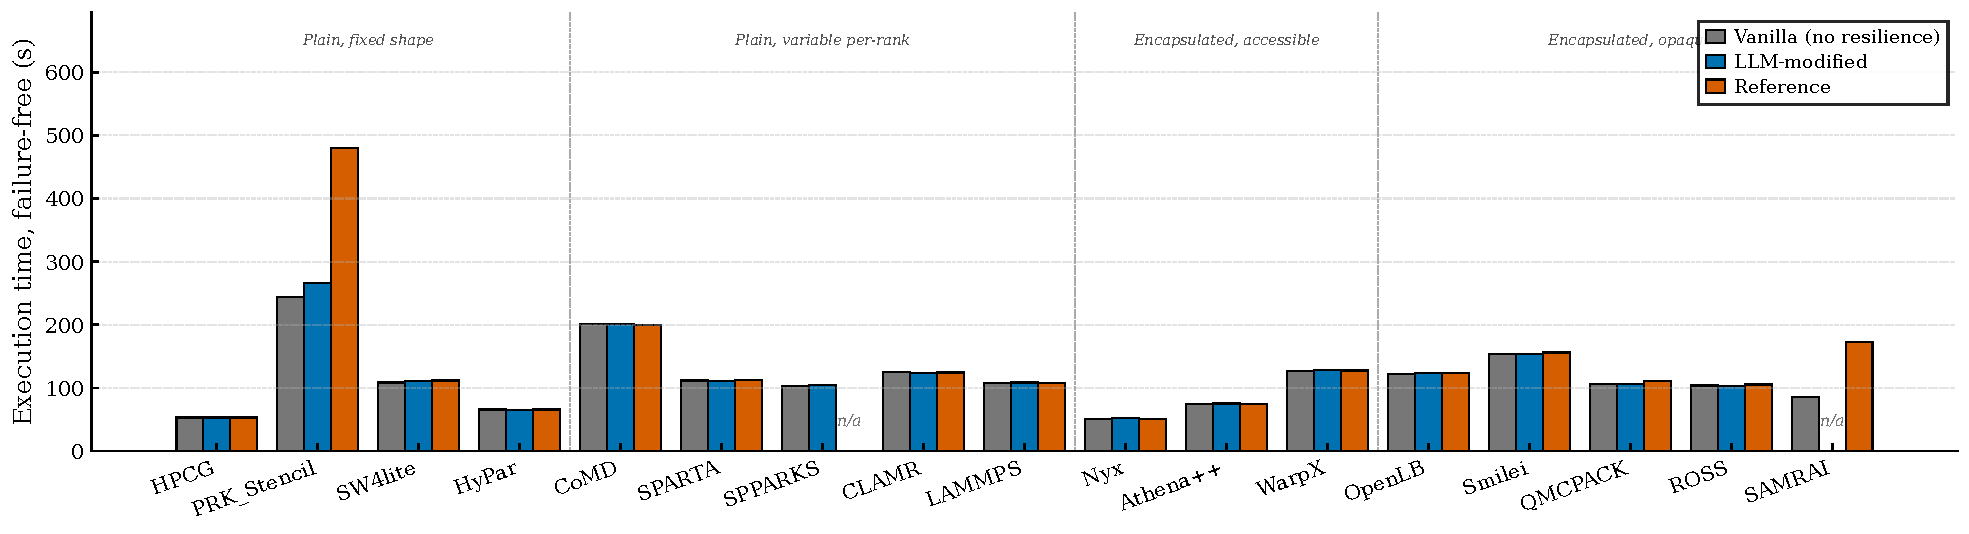
\includegraphics[width=\columnwidth]{Figures/fast_tier_compare_walltime_failure_free.pdf}
  \caption{Per-app average execution time under the failure-free scenario.}
  \label{fig:ff}
\end{figure}

\begin{figure}[t]
  \centering
  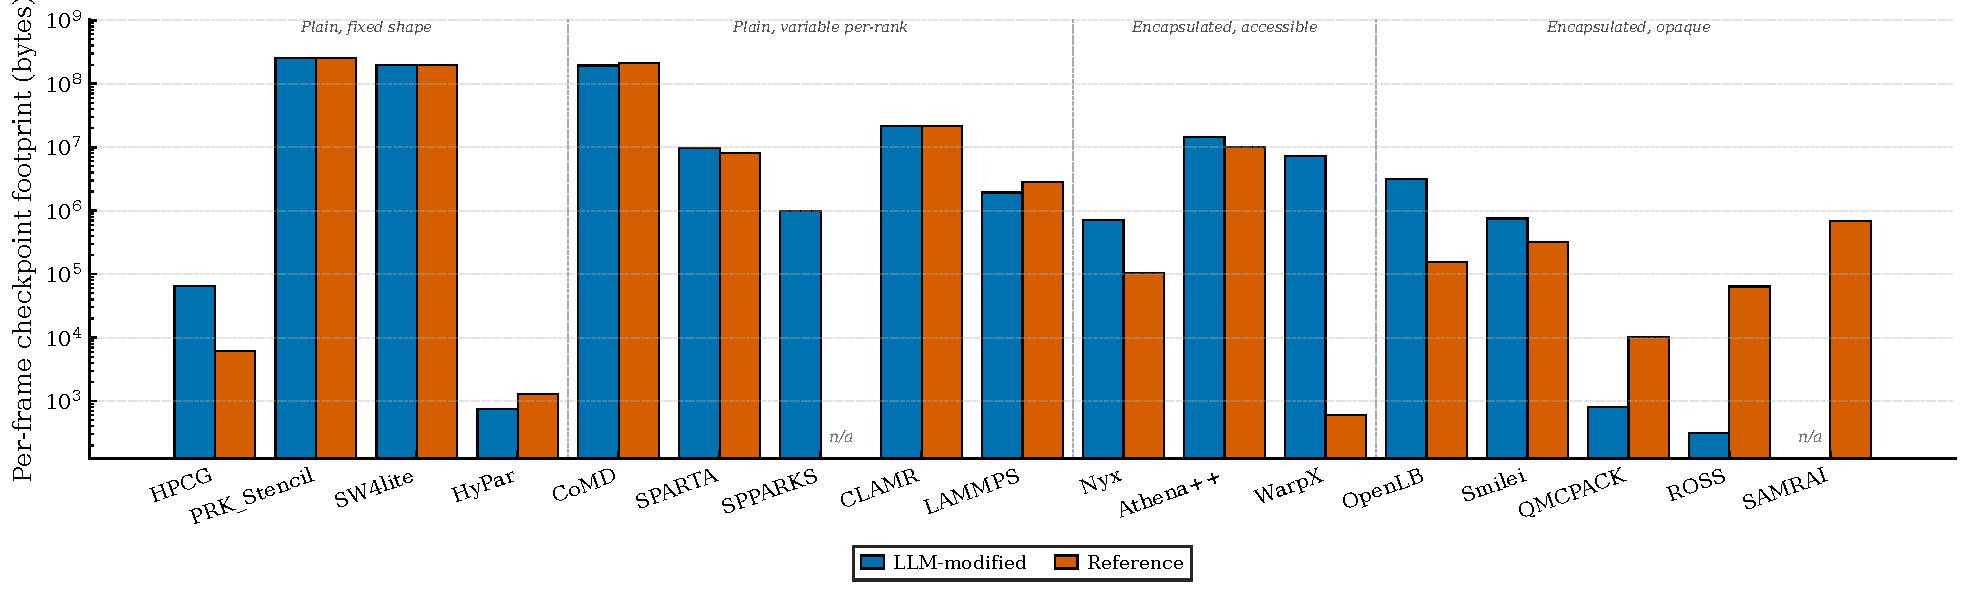
\includegraphics[width=\columnwidth]{Figures/fast_tier_compare_checkpoint_per_frame.pdf}
  \caption{Payload size of a full recoverable checkpoint.}
  \label{fig:frame}
\end{figure}

\medskip
\noindent\textbf{Overhead: Runtime and Storage.}
\autoref{fig:ff} shows an important result for the sixteen LLM-baseline cells that survived the trust gate: \textit{the LLM-generated checkpoint instrumentation imposes essentially zero failure-free overhead}. Fourteen of those sixteen apps fall within $\pm 2\%$ of vanilla wall time (range $-1.1\%$ for CLAMR to $+1.9\%$ for SW4lite, with Smilei joining at $-0.2\%$ post-2026-05-15 honest-redo), well inside measurement noise. Nyx falls in the moderate band ($+2.6\%$, an over-frequent VeloC commit cadence). Only PRK\_Stencil shows a larger overhead at $+9.2\%$, attributable to the chosen checkpoint cadence on its tight stencil loop. The LLM bars track the upstream reference closely on every app, so the generated code matches a human-engineered native implementation. Bars for SAMRAI render as ``n/a'' because the LLM baseline remains UNTRUSTED (gaming; see cross-cutting observations).

\autoref{fig:frame} shows full-checkpoint sizes spanning many orders of magnitude, from per-frame footprints under 1~KB (HyPar 744~B, QMCPACK 40~B, ROSS 312~B, Smilei 256~B) up to gigabytes (CoMD's 194~MB and SW4lite's 196~MB and PRK\_Stencil's 257~MB). LLM and reference agree on the order of magnitude on most apps. The most informative divergence is WarpX, where the LLM-generated checkpoint (44~MB per run) is $\sim$26$\times$ smaller than the upstream AMReX-native reference (1.13~GB per run). We dissected the difference: per AMReX checkpoint directory, the reference saves nine field MultiFabs (\texttt{Ex\_fp}, \texttt{Ey\_fp}, \texttt{Ez\_fp}, \texttt{Bx\_fp}, \texttt{By\_fp}, \texttt{Bz\_fp}, \texttt{jx\_fp}, \texttt{jy\_fp}, \texttt{jz\_fp}, $\sim$1.3~MB each) plus header metadata, totalling $\sim$11~MB; we sampled the \texttt{j*\_fp} files on disk and confirmed they are pure zeros for the validation input (vacuum, no particles, so $j = q n v \equiv 0$). The LLM correctly identifies that current density is statically derivable in this regime and saves only the six EM-field components ($\sim$7~MB per frame). The remaining factor of the size gap comes from retention policy: VeloC's \texttt{max\_versions=3} with three scratch tiers caps the LLM at six on-disk frames per bench run, while AMReX's native checkpoint retains every chk dir written, accumulating roughly an order of magnitude more frames over the same run. Combined ($\sim$1.6$\times$ per-frame $\times$ $\sim$16$\times$ retained frames) the two effects produce the observed 26$\times$ reduction. \textbf{[TODO: 1 of 17 reference checkpoints (SPPARKS) still reports as ``n/a'' because the SPPARKS reference uses a text visualization \texttt{dump} rather than its native \texttt{stitch} format; switch the patch to \texttt{stitch} dumps before camera-ready.]}

% \subsection{Resiliency}

\begin{figure}[t]
  \centering
  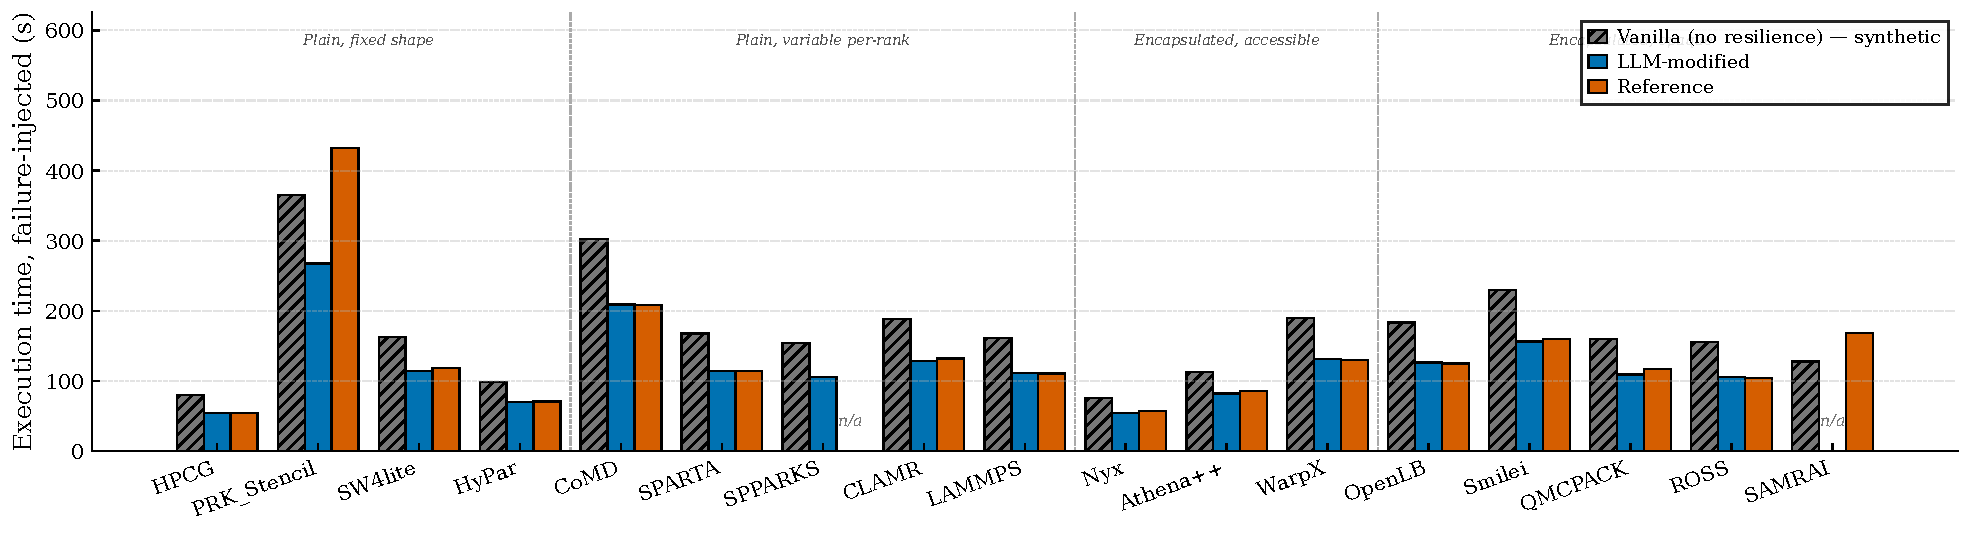
\includegraphics[width=\columnwidth]{Figures/fast_tier_compare_walltime_failure_injected.pdf}
  \caption{Per-app end-to-end execution time with a failure injected mid-run.
  % The binary re-launches after failures. LLM-modified and reference binary detect existing checkpoint files and resume while vanilla has to restart from scratch.
  }
  \label{fig:once}
\end{figure}

\medskip
\noindent\textbf{Resilience.}
\autoref{fig:once} shows per-app end-to-end runtime when the validator kills one MPI rank mid-run, then restarts the app. Of the sixteen LLM baselines that survived the trust gate, fifteen recover with a once / failure-free ratio between 1.01$\times$ and 1.09$\times$ (Nyx 1.05$\times$ post-2026-05-14 and Smilei 1.02$\times$ post-2026-05-15 join this band as honest-redos). Both the LLM and reference recover within roughly one third of the wall-clock penalty paid by the vanilla baseline, which has no checkpoint protection and must restart from scratch. The lone outlier is OpenLB at 1.41$\times$, which spends a disproportionate share of the post-failure run rebuilding its lattice geometry through the same expensive initialization path the vanilla pays at startup. Apart from this, the chart is operational evidence the LLM-generated code does real recovery work: detecting checkpoint files, restoring state, and resuming with overhead bounded by the checkpoint cadence rather than by the size of the original computation. Bars for SAMRAI render as ``n/a'' for the LLM (gaming demotion; see cross-cutting observations).

% =====================================================================
\section{Conclusion and Future Work}
\label{sec:conclusion}
% =====================================================================

This paper investigates whether frontier LLM coding agents can automate end-to-end checkpoint/restart integration for existing MPI scientific applications. Across seventeen applications with diverse domains (1K to 627K LOC), data structures, and checkpointing patterns, the agent generated working resilient implementations without human intervention after the initial prompt. The generated code achieved near-zero failure-free overhead on sixteen of seventeen applications, recovered from injected failures with performance close to upstream native implementations on every app where the comparison is available, and converged in under two hours per application. These results suggest that LLM-driven resilience engineering can substantially reduce the expert effort required to add production-grade fault tolerance to a meaningful subset of HPC applications.

Future work should improve the robustness, scalability, and usability of this approach. Specialized pipelines with resilience-specific skills, source-code summarization, checkpoint-state analysis, and targeted validation feedback could reduce cost and improve reliability. Broader evaluations are needed for repeated failures, realistic I/O environments, multi-node executions, and applications with more irregular or distributed state. Finally, generated checkpoint code should become easier to audit, maintain, and integrate into production workflows so that automated resilience generation can be used safely in practice.

\bibliographystyle{IEEEtran}
\bibliography{references}

% \section*{References}

% Please number citations consecutively within brackets \cite{b1}. The 
% sentence punctuation follows the bracket \cite{b2}. Refer simply to the reference 
% number, as in \cite{b3}---do not use ``Ref. \cite{b3}'' or ``reference \cite{b3}'' except at 
% the beginning of a sentence: ``Reference \cite{b3} was the first $\ldots$''

% Number footnotes separately in superscripts. Place the actual footnote at 
% the bottom of the column in which it was cited. Do not put footnotes in the 
% abstract or reference list. Use letters for table footnotes.

% Unless there are six authors or more give all authors' names; do not use 
% ``et al.''. Papers that have not been published, even if they have been 
% submitted for publication, should be cited as ``unpublished'' \cite{b4}. Papers 
% that have been accepted for publication should be cited as ``in press'' \cite{b5}. 
% Capitalize only the first word in a paper title, except for proper nouns and 
% element symbols.

% For papers published in translation journals, please give the English 
% citation first, followed by the original foreign-language citation \cite{b6}.

% \begin{thebibliography}{00}
% \bibitem{b1} G. Eason, B. Noble, and I. N. Sneddon, ``On certain integrals of Lipschitz-Hankel type involving products of Bessel functions,'' Phil. Trans. Roy. Soc. London, vol. A247, pp. 529--551, April 1955.
% \bibitem{b2} J. Clerk Maxwell, A Treatise on Electricity and Magnetism, 3rd ed., vol. 2. Oxford: Clarendon, 1892, pp.68--73.
% \bibitem{b3} I. S. Jacobs and C. P. Bean, ``Fine particles, thin films and exchange anisotropy,'' in Magnetism, vol. III, G. T. Rado and H. Suhl, Eds. New York: Academic, 1963, pp. 271--350.
% \bibitem{b4} K. Elissa, ``Title of paper if known,'' unpublished.
% \bibitem{b5} R. Nicole, ``Title of paper with only first word capitalized,'' J. Name Stand. Abbrev., in press.
% \bibitem{b6} Y. Yorozu, M. Hirano, K. Oka, and Y. Tagawa, ``Electron spectroscopy studies on magneto-optical media and plastic substrate interface,'' IEEE Transl. J. Magn. Japan, vol. 2, pp. 740--741, August 1987 [Digests 9th Annual Conf. Magnetics Japan, p. 301, 1982].
% \bibitem{b7} M. Young, The Technical Writer's Handbook. Mill Valley, CA: University Science, 1989.
% \end{thebibliography}
% \vspace{12pt}
% \color{red}
% IEEE conference templates contain guidance text for composing and formatting conference papers. Please ensure that all template text is removed from your conference paper prior to submission to the conference. Failure to remove the template text from your paper may result in your paper not being published.

\end{document}
